\section{Evaluation}\label{sec:evaluation}
\subsection{Setup}
We ran the detector for one week on three pipelines operated by an analytics company: order events (P1), application logs (P2) and sensor telemetry (P3). Windows were one minute long. To measure detection we injected 48 changes of four kinds into copies of the streams, each affecting between 2\% and 100\% of records. As a baseline we compared complete signatures between windows, which is exact but must ship every distinct signature to the coordinator.

\subsection{Results}
Table~\ref{tab:results} lists the outcome per pipeline. The detector found 46 of the 48 injected changes; the two it missed affected 2\% of records in P2, the pipeline with the most varied structure. It raised two false alarms in the week, both during a deployment that briefly doubled the share of one record type.

\begin{table}[t]
  \caption{Detection results for one week per pipeline. Overhead is the increase in processing time compared with the pipeline without the detector.}
  \label{tab:results}
  \centering
  \begin{tabular}{lrrrrr}
    \toprule
    Pipeline & Events/h & Injected & Detected & False alarms & Overhead \\
    \midrule
    P1 Orders    &  3.1 M & 16 & 16 & 0 & 1.2\% \\
    P2 Logs      & 10.4 M & 16 & 14 & 2 & 2.6\% \\
    P3 Telemetry &  6.7 M & 16 & 16 & 0 & 1.7\% \\
    \midrule
    Total        & 20.2 M & 48 & 46 & 2 & 1.8\% \\
    \bottomrule
  \end{tabular}
\end{table}

Fig.~\ref{fig:delay} shows how quickly a change is reported as the stream grows. Because sketches are merged rather than recomputed, the delay of our detector falls below one second after three million events, whereas the full comparison stays above one second throughout.

\begin{figure}[t]
  \centering
  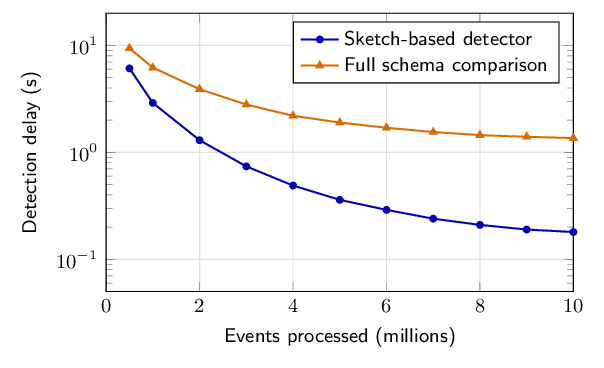
\includegraphics[width=0.8\textwidth]{figures/detection-delay.png}
  \caption{Time from an injected change to its report, as a function of the number of events processed.}
  \label{fig:delay}
\end{figure}

\subsection{Discussion}
The sketch does not say which field changed, only that the structure did. In practice the report includes the five counters with the largest difference, and an engineer resolved the field from them in under a minute in all but one case. Changes confined to rare record types remain hard to detect with any fixed threshold.
